\chapter{ARSITEKTUR SISTEM}

Jika membahas arsitektur sistem, maka akan ada beberapa diagram yang terbentuk untuk memudahkan dalam penjelasan sebuah sistem. Penggambaran diagram arsitektur sistem ini berkembang mengikuti model pemrogramannya, dimana dahulu ada yang dikenal dengan \textit{flow-chart} yang menggambarkan alur proses sebuah sistem aplikasi berjalan, mulai dari awal, sampai sistem aplikasi tersebut ditutup dan selesai digunakan, karena memang model pemrograman pada saat ini berbentuk prosedural. 

Namun berkembangnya jaman, dikenal istilah pemrograman berorientasi objek, yang salah satu bahasa pemrogramannya adalah Java. Dengan menggunakan Java, maka diagram \textit{flow-chart} tidak akan bisa melakukan penggambaran alurnya karena pola pada pemrograman berorientasi objek selalu melompat dari satu kelas ke kelas yang lain, dari satu \textit{method} ke \textit{method} yang lain. Maka dibutuhkan penggambaran desain arsitektur yang lain selain \textit{flow-chart}, salah satunya adalah \textit{Unified Modelling Language} (UML).

UML sendiri sebetulnya hanya menggambarkan 2 (dua) sudut pandang dalam pemodelan sistem, yaitu :

\begin{itemize}
  \item \textit{Static view}, yang menekankan pada struktur sistem yang bersifat statis seperti objek, operasi, dan relasi.
  
  \item \textit{Dynamic view}, yang menekankan pada sifat atau tingkah laku dari sistem yang menunjukkan interaksi antar objek didalamnya.
\end{itemize}

\section{Diagram \textit{Use-Case}}

Hal yang pertama digambarkan adalah skenario penggunaan aplikasi secara umum, akan berangkat dari diagram \textit{use-case} seperti pada gambar \ref{fig:uml-use-case} :

\begin{figure}[H]
  \centering
  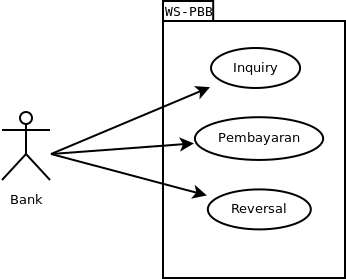
\includegraphics[width=0.5\textwidth]{./resources/uml/uml-use-case}
  \caption{Diagram \textit{use-case}}
  \label{fig:uml-use-case}
\end{figure}

Dari diagram \textit{use-case} diatas, skenarionya adalah bahwa Bank sebagai tempat pembayaran dapat melakukan \textit{request} pada ketiga hal yang disediakan oleh \textit{web services} PBB di DPPK. yaitu :

\begin{itemize}
  \item \textit{Inquiry}
  \item Pembayaran
  \item Reversal
\end{itemize}

Untuk melihat masing-masing proses pada skenario diatas, ada pada diagram \textit{activity} yang dibahas pada bagian selanjutnya. 

\section{Diagram \textit{Activity}}

Diagram \textit{activity} ini akan menunjukan aktivitas yang terjadi untuk setiap skenario pada diagram \textit{use-case}. Berikut skema diagram dari masing-masing skenario yang terbagi menjadi 3 (tiga) diagram berdasarkan jumlah skenario pada diagram \textit{use-case} :

\subsection{Diagram \textit{Activity} Untuk \textit{Inquiry}}

Bagan diagram \textit{activity} untuk \textit{inquiry} ini seperti ditunjukan pada gambar \ref{fig:act-inquiry} :

\begin{figure}[H]
  \centering
  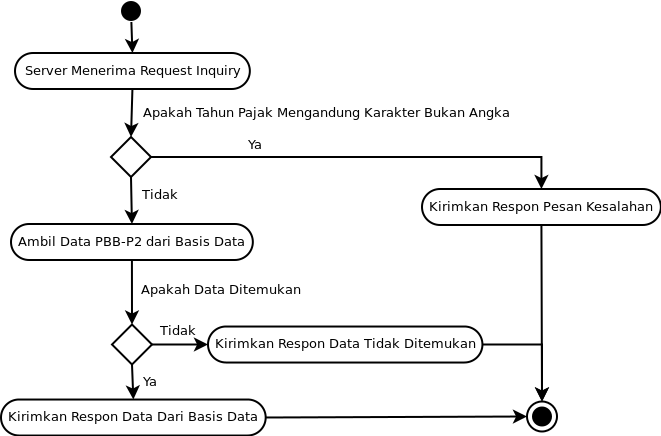
\includegraphics[width=0.8\textwidth]{./resources/uml/uml-act-inquiry}
  \caption{Diagram \textit{Activity} untuk \textit{Inquiry}}
  \label{fig:act-inquiry}
\end{figure}

Aktivitas akan dimulai dari lingkaran penuh di atas, yang kemudian didahului oleh \textit{client} yang melakukan \textit{request} untuk \textit{inquiry} data PBB-P2, hal yang pertama dilakukan adalah melakukan pemeriksaan informasi tahun pajak yang diminta, apakah mengandung karakter atau tidak.

Bila Tahun pajak terisi dengan angka yang wajar, maka aplikasi \textit{web services} akan melakukan koneksi dengan basis data SISMIOP untuk mengambil informasi-informasi yang dibutuhkan oleh \textit{client}.

Bila data tidak ditemukan dalam basis data, maka aplikasi \textit{web services} akan mengirimkan informasi kepada \textit{client} bahwa data yang diminta tidak ditemukan, namun bila data ditemukan, maka disusun dalam format JSON dan dikirimkan ke \textit{client} sebagai respon atas \textit{request} tersebut.

Sampai sini aktivitas selesai.

\subsection{Diagram \textit{Activity} Untuk Pencatatan Pembayaran}

Diagram \textit{activity} untuk melakukan pencatatan pembayaran dapat dilihat seperti pada gambar \ref{fig:act-bayar} :

\begin{figure}[H]
  \centering
  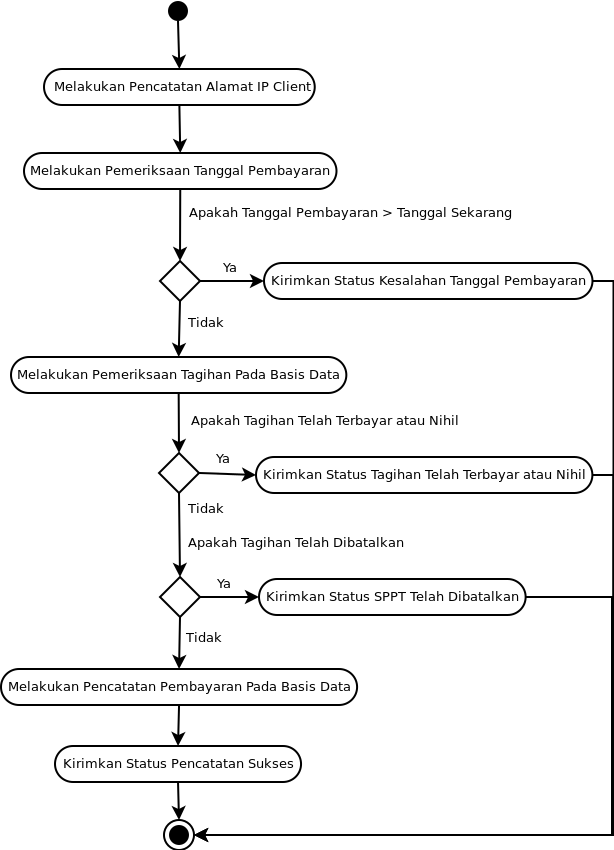
\includegraphics[width=0.8\textwidth]{./resources/uml/uml-act-bayar}
  \caption{Diagram \textit{Activity} Untuk Pencatatan Pembayaran}
  \label{fig:act-bayar}
\end{figure}

Aktivitas pencatatan pembayaran diawali pada saat \textit{client} melakukan \textit{request} pembayaran SPPT PBB-P2, \textit{server web services} akan melakukan pencatatan alamat IP darimana \textit{request} tersebut berasal.

Kemudian \textit{server} akan melakukan pemeriksaan terhadap tanggal pembayaran, apabila tanggal pembayaran melebihi tanggal saat dilakukannya proses pencatatan pembayaran, maka \textit{server} akan mengirimkan status kesalahan tanggal pembayaran ke \textit{client}, dan aktivitas selesai, namun bila tanggal pembayaran kurang dari atau sebelum hari dilakukannya proses pencatatan, maka aktivitas berlanjut ke proses berikutnya.

Pada tahap ini \textit{server} melakukan pemeriksaan tagihan pada basis data, apakah kondisi objek pajak (yang teridentifikasi dari nomor objek pajak) sudah terbayar atau belum, atau tagihannya nihil (tidak ada pajak yang terhutang), bila ya, maka \textit{server} akan mengirimkan status ke \textit{client} bahwa objek yang diminta telah terbayar atau merupakan objek yang piutangnya nihil. bila tidak, maka proses berlanjut.

Proses akhir dari aktivitas ini adalah melakukan pencatatan pembayaran pada basis data, kemudian mengirimkan status bahwa pencatatan tersebut telah selesai. Sampai sini aktivitas telah sampai pada ujung prosesnya.

\subsection{Diagram \textit{Activity} Untuk \textit{Reversal}}

Diagram \textit{activity} untuk melakukan proses \textit{reversal} adalah sebagaimana ditunjukkan pada gambar \ref{fig:act-reversal} :

\begin{figure}[H]
  \centering
  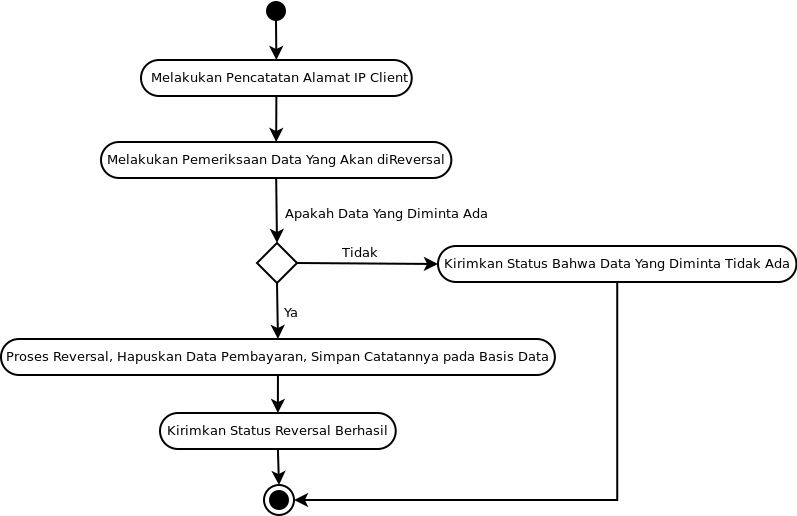
\includegraphics[width=0.8\textwidth]{./resources/uml/uml-act-reversal}
  \caption{Diagram \textit{Activity} Untuk Proses \textit{Reversal}}
  \label{fig:act-reversal}
\end{figure}

Seperti kedua aktivitas sebelumnya, hal yang pertama dilakukan adalah melakukan pencatatan alamat IP dari \textit{client}.

Kemudian melakukan pemeriksan data yang akan direversal, terutama terhadap Nomor Transaksi Pajak Daerah (NTPD) sebagai identitas sebuah transaksi. Apabila data NTPD ini salah, maka \textit{server} akan mengirimkan status kegagalan \textit{reversal} karena data yang diminta tidak ada. Bila data ada, maka melanjutkan ke proses berikutnya.

Langkah berikutnya adalah melakukan pencatatan \textit{request reversal} dan mengirimkan status ke \textit{client} bahwa \textit{reversal} yang diminta telah berhasil dilakukan.

Sampai sini aktivitas \textit{reversal} selesai.

Dari diagram \textit{use-case} dan diagram \textit{activity} telah didapat gambaran umum dari sistem aplikasi yang akan dibangun. Diagram-diagram berikutnya akan lebih detail membahas teknis bagaimana sistem bekerja.

\section{Diagram \textit{Class}}

Pada diagram \textit{class} ini, akan membahas detail dari tiap kelas pembentuk sistem aplikasi \textit{web services} secara keseluruhan. Karena akan menggunakan \textit{framework} Spring yang tentunya memiliki spesifikasi tersendiri, maka untuk memperjelas gambar diagram \textit{class} akan dibagi menjadi beberapa bagian, yaitu :

\begin{enumerate}
  \item Bagian Konfigurasi
  
  Bagian ini adalah kelas-kelas pembentuk konfigurasi \textit{framework} Spring sehingga aplikasi dapat dengan mudah dibangun tanpa perlu memikirkan detail teknis bagaimana Rest harus bekerja. Diagram \textit{class} dari bagian konfigurasi ini seperti ditunjukkan pada gambar \ref{fig:uml-class-konfig} :
  
  \begin{figure}[H]
    \centering
    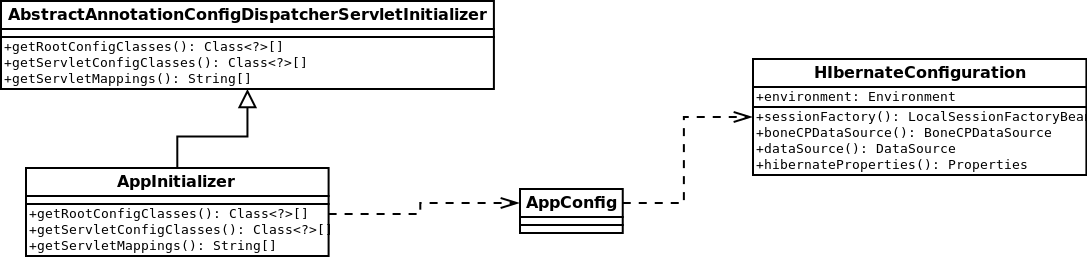
\includegraphics[width=1\textwidth]{./resources/uml/uml-class-konfig}
    \caption{Diagram \textit{Class} Bagian Konfigurasi \textit{Framework} Spring}
    \label{fig:uml-class-konfig}
  \end{figure}
  
  Kelas-kelas inilah yang nantinya mengatur \textit{services} dan konfigurasi koneksi dengan basis data. Awalnya \textit{servlet container} akan memanggil kelas AppInitializer hasil turunan dari kelas atau \textit{interface} AbstractAnnotationConfigDispatcherServletInitializer. Kelas AppInitializer ini membutuhkan kelas AppConfig untuk melakukan Konfigurasi khusus terkait struktur \textit{framework} Spring yang digunakan. Kelas AppConfig ini pun melakukan pemanggilan kelas HibernateConfiguration untuk melakukan konfigurasi komunikasi dengan \textit{server} basis data.
 
  \item Bagian \textit{Inquiry}
  
  Kelas-kelas pada bagian \textit{inquiry} ini, beberapa akan muncul pada bagian transaksi pembayaran ataupun \textit{reversal} karena kelas-kelas tersebut memiliki fungsi yang sama dalam siklus melayani \textit{request} dari \textit{client}. Kelas-kelas pada bagian \textit{inquiry} ini akan terlihat seperti pada gambar \ref{fig:uml-class-inquiry}
  
  \begin{figure}[H]
    \centering
    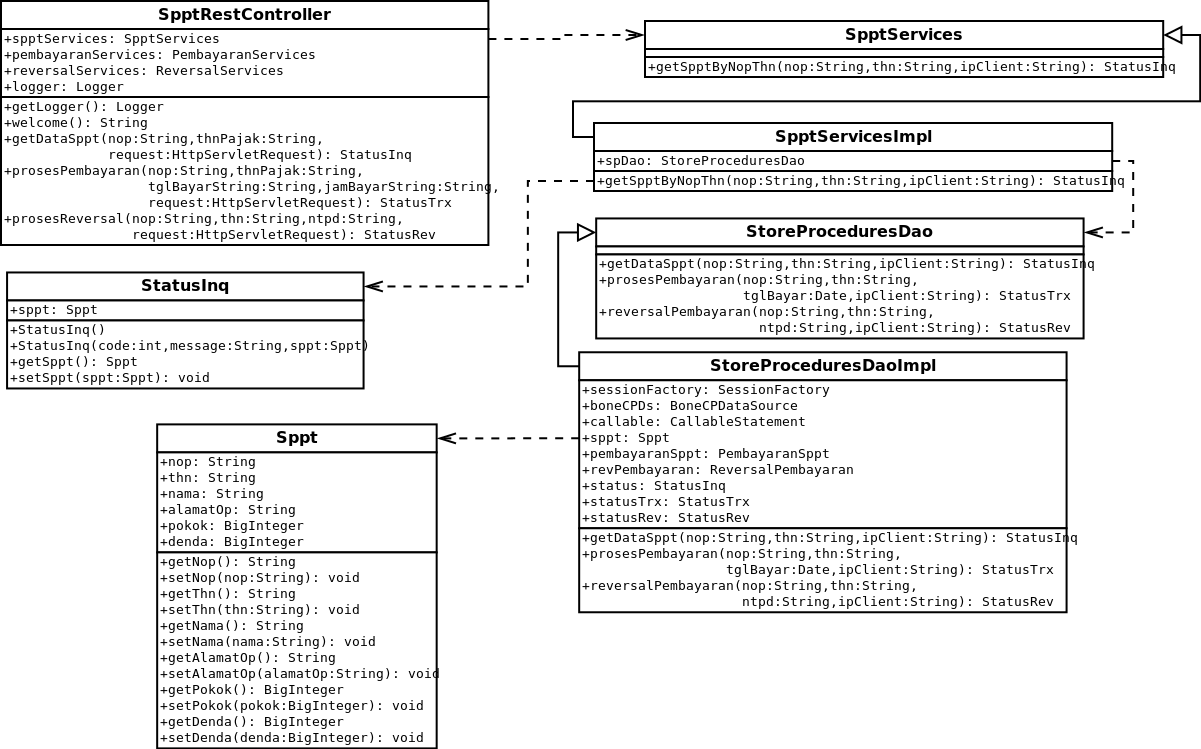
\includegraphics[width=1\textwidth]{./resources/uml/uml-class-inquiry}
    \caption{Diagram \textit{Class} Bagian \textit{Inquiry}}
    \label{fig:uml-class-inquiry}
  \end{figure}
  
  Kelas yang akan menjadi titik awal datangnya sebuah \textit{request} dari \textit{client} adalah kelas SpptRestController, kelas ini yang nantinya akan memilih apakah \textit{request client} adalah \textit{inquiry}, transaksi pembayaran, atau permohonan \textit{reversal}. Kelas SpptRestController ini pula yang nantinya mengirimkan pada \textit{service} yang berkaitan.
  
  Berkaitan dengan bagian \textit{inquiry}, maka begitu ada \textit{request inquiry} dikirimkan oleh \textit{client} dan diterima \textit{server} maka kemudian dipanggil \textit{interface} SpptServices, yang pada struktur kali ini diimplementasikan oleh kelas SpptServicesImpl.
  
  Karena \textit{framework} yang digunakan adalah Spring, maka diperlukan beberapa bagian berdasarkan fungsi utamanya. Fungsi dari masing-masing kelas yang berada pada \textit{framework} Spring yaitu :
  
  \begin{itemize}
    \item \textit{Domain Object}. Kelas-kelas yang memiliki fungsi ini mewakili struktur data persis seperti pada basis data. Penggunaan kelas-kelas pada \textit{domain object} diperlukan karena :
    
    \begin{enumerate}[1)]
      \item Kode program jadi lebih mudah dimengerti dan dipelihara.
      \item Karena Java merupakan bahasa yang \textit{strongly-typed} dan harus di-\textit{compile} terlebih dahulu, akan memudahkan pemeriksaan \textit{bug} pada saat \textit{compile} dibandingkan saat \textit{runtime} atau berjalannya aplikasi.
      \item Memisahkan lapisan data dan antarmuka / \textit{interface}. Apabila ada perubahan skema pada basis data tetapi fitur pada tampilan antarmuka tidak berubah, maka cukup dilakukan perubahan pada lapisan data / \textit{domain object}-nya saja.
      \item Pustaka siap pakai untuk validasi. Di Java, ada pustaka yang berguna untuk melakukan validasi, yaitu JSR-303. Terhadap validasi data yang akan dimasukkan ke dalam basis data, kita tidak perlu melakukan pengecekan seperti contoh kode berikut :
      
      \begin{lstlisting}[language=java]
      if(mydata.getId() == null)
      \end{lstlisting}
      
      Melainkan cukup dengan kode berikut :
      
      \begin{lstlisting}[language=java]
      @NotNull private String Id;
      \end{lstlisting}
    \end{enumerate}
    
    \item \textit{Interface Business Services}
    
    Kelas-kelas pada fungsi ini hanya berupa definisi daftar fitur yang disediakan oleh aplikasi. Seluruh implementasi dikelas ini belum terisi, oleh karena itu dinamakan \textit{interface}. Beberapa alasan penggunaan \textit{interface} atau kelas-kelas abstrak atau tanpa implementasi ini adalah sebagai berikut :
    
    \begin{itemize}
      \item Pada saat membangun sebuah aplikasi \textit{client-server}, maka cukup dengan memberikan kelas-kelas pada \textit{domain object} dan \textit{interface} ini pada \textit{programmer} yang membangun sisi \textit{client}, tanpa perlu menyertakan implementasi dari \textit{interface} yang biasanya cukup besar, aplikasi dapat saling berkomunikasi.
      
      \item Pada saat ada peralihan atau perubahan implementasi perangkat lunak basis data, maka aplikasi disisi \textit{client} tidak perlu berubah.
      
      \item Fitur \textit{declarative transaction} yang dimiliki Spring akan lebih optimal bekerja bila dipisahkan antara \textit{interface} dengan implementasinya.
    \end{itemize}
    
    \item \textit{Implementasi Business Services}
    
    Ini adalah bagian dari implementasi \textit{interface business services}. Jika pada \textit{interface} berisi fitur abstrak, pada bagian ini sudah ada implementasi konkrit untuk masing-masing fitur yang telah didefinisikan pada \textit{interface}. Karena sistem aplikasi akan menggunakan Spring Data JPA, maka diperlukan kelas-kelas lain selain \textit{business services}, yaitu kelas-kelas implementasi \textit{Data Access Object} (DAO).
  \end{itemize}
  
  Implementasi dari kelas SpptServicesImpl akan mengembalikan kelas StatusInq sebagai respon terhadap \textit{request} yang telah sampai ke \textit{server}. Kelas SpptServicesImpl membutuhkan paket kelas DAO berupa \textit{interface} StoreProceduresDao untuk melakukan komunikasi dengan basis data. Implementasi dari \textit{interface} StoreProceduresDao ini adalah kelas StoreProceduresDaoImpl dimana implementasi didalamnya akan menggunakan kelas Sppt untuk menyimpan atau menampung nilai-nilai yang dihasilkan dari pemanggilan \textit{store procedure} pada basis data. Yang pada akhirnya akan dikembalikan kelas Sppt ini dalam bentuk yang terbungkus dalam kelas StatusInq.
  
  \item Bagian Transaksi Pembayaran
  
  Kelas-kelas pembentuk bagian transaksi pembayaran ini adalah kelas-kelas yang saling berhubungan agar \textit{request} transaksi pembayaran dapat diproses sempurna oleh \textit{server}. Kelas-kelas pembentuk bagian transaksi pembayaran ini adalah seperti terlihat pada gambar \ref{fig:uml-class-bayar} :
  
  \begin{figure}[H]
    \centering
    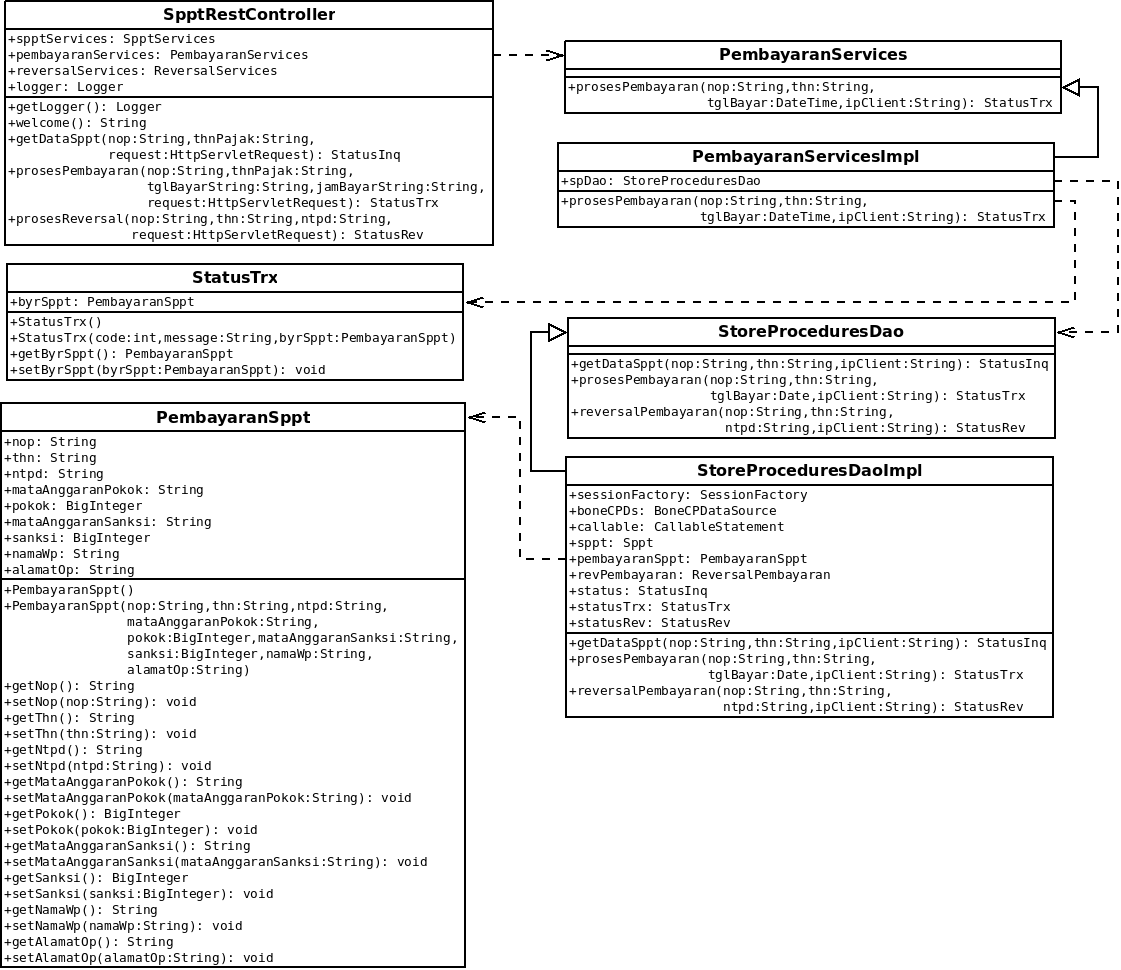
\includegraphics[width=1\textwidth]{./resources/uml/uml-class-bayar}
    \caption{Diagram \textit{Class} Untuk Bagian Pembayaran}
    \label{fig:uml-class-bayar}
  \end{figure}
  
  Seperti bagian sebelumnya, kelas SpptRestController yang sama muncul di bagian ini karena dari kelas inilah titik awal sebuah \textit{request} dari \textit{client} dimulai.
  
  Yang berbeda dari bagian ini adalah kelas-kelas PembayaranServices dan PembayaranServicesImpl sebagai \textit{interface} dan kelas implementasinya yang dibutuhkan oleh \textit{framework} Spring, kemudian ada kelas StatusTrx sebagai pembungkus respon yang nantinya dikirimkan ke \textit{client}, serta kelas PembayaranSppt untuk menampung informasi yang datang dari basis data hasil dari pemanggilan DAO dari kelas StoreProceduresDaoImpl yang sama seperti pada bagian \textit{inquiry}. pada bagian transaksi pembayaran ini pun, kelas PembayaranSppt sebagai bahan respon atas \textit{request} dari \textit{client} akan dibungkus dengan kelas \textit{StatusTrx} agar informasi yang sampai ke \textit{client} dapat lebih jelas.
  
  \item Bagian \textit{Reversal}
  
  Kelas-kelas pembentuk bagian \textit{reversal} ini berfungsi untuk melakukan \textit{reversal} transaksi yang sebelumnya telah terjadi. Kelas-kelas pada bagian ini seperti terlihat pada gambar \ref{fig:uml-class-rev} :
  
  \begin{figure}[H]
    \centering
    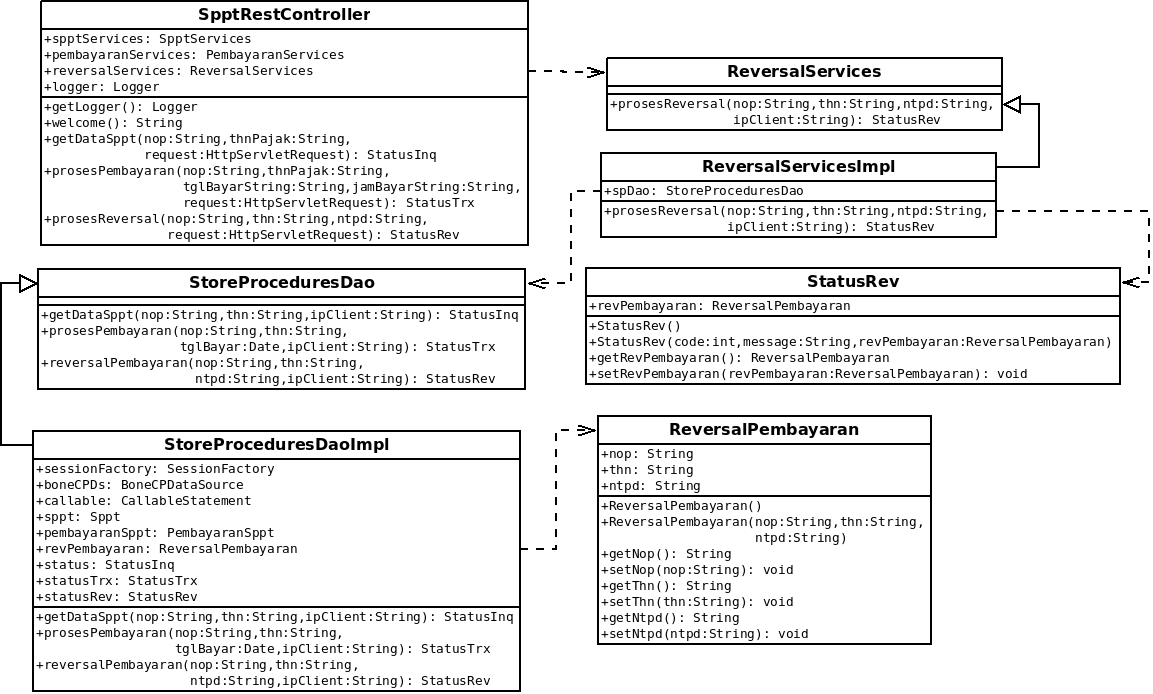
\includegraphics[width=1\textwidth]{./resources/uml/uml-class-rev}
    \caption{Diagram \textit{Class} Yang Berhubungan Dengan Proses \textit{Reversal}}
    \label{fig:uml-class-rev}
  \end{figure}
  
  Seperti pada bagian-bagian sebelumnya, kelas SpptRestController tetap ada sebagai titik awal masuknya sebuah \textit{request} yang akan diproses. Kemudian karena \textit{request} yang diterima berupa proses \textit{reversal} maka akan berhubungan dengan \textit{interface} ReversalServices dan kelas ReversalServicesImpl untuk mengikuti aturan dari \textit{framework} Spring.
  
  Sebagai penghubung komunikasi antara aplikasi dengan basis data, tetap menggunakan \textit{interface} StoreProceduresDao dengan kelas StoreProceduresDaoImpl sebagai implementasinya. Sebagai bahan respon, data-data hasil pengambilan dari basis data akan ditampung pada kelas ReversalPembayaran dengan dibungkus kelas StatusRev untuk mempermudah menambahkan informasi-informasi sukses atau gagalnya operasi yang terjadi pada \textit{server}.
  
\end{enumerate}

\section{Diagram \textit{Sequence}}

Untuk penjelasan diagram \textit{sequence} ini pun, agar diagram terlihat jelas alurnya, maka perlu dipecah menjadi beberapa bagian. Agar lebih mudah memahami prosesnya, diagram akan dipecah seperti pada diagram \textit{class} yaitu hanya saja untuk diagram \textit{sequence} ini akan berbentuk skenario-skenario sebagai berikut :

\subsection{Skenario Konfigurasi \textit{Spring Framework}}

Bagian ini akan menjelaskan bagaimana alur dari awal \textit{server} melakukan inisialisasi sistem, sampai kepada tahap \textit{server} siap menerima \textit{request}. Diagram \textit{sequence} untuk keadaan ini dapat dilihat seperti pada gambar \ref{fig:uml-seq-konf} :
  
  \begin{figure}[H]
    \centering
    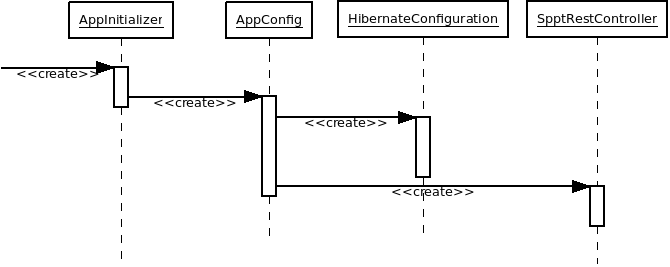
\includegraphics[width=1\textwidth]{./resources/uml/uml-seq-konf}
    \caption{Diagram \textit{Sequence} Untuk Konfigurasi dan Inisialisasi}
    \label{fig:uml-seq-konf}
  \end{figure}
  
  Pada awalnya \textit{servlet container} akan melakukan inisialisasi kelas AppInitializer yang merupakan turunan dari kelas AbstractAnnotationConfigDispatcherServletInitializer, objek AbstractAnnotationConfigDispatcherServletInitializer ini merupakan \textit{interface} yang disediakan \textit{framework} Spring untuk tempat memulai melakukan inisialisasi.
  
  Lalu kelas AppInitializer melakukan inisialisasi terhadap kelas AppConfig untuk melakukan konfigurasi-konfigurasi yang diperlukan agar sistem aplikasi dapat bekerja dengan baik. Salah satu diantaranya adalah melakukan inisialisasi terhadap kelas SpptRestController, kelas inilah yang nantinya melakukan seleksi \textit{request} dan mengirimkan pada kelas \textit{service} yang berkaitan.
  
  Selain melakukan inisialisasi terhadap kelas SpptRestController, kelas AppConfig pun melakukan inisialisasi terhadap kelas HibernateConfiguration. Kelas HibernateConfiguration ini mempersiapkan koneksi dengan basis data dengan menyediakan modul-modul yang dapat digunakan pada sistem aplikasi nantinya.
  
\subsection{Skenario \textit{Inquiry} Gagal Karena Tahun Pajak Bukan Angka}

Skenario ini akan menggambarkan kondisi dimana \textit{client} mengirimkan \textit{request inquiry}, namun setelah diseleksi oleh \textit{server} terdapat karakter bukan angka pada tahun pajak yang di-\textit{request}. Diagram \textit{sequence} dari skenario ini dapat dilihat pada gambar \ref{fig:uml-seq-inq-thn-not-valid} :

\begin{figure}[H]
  \centering
  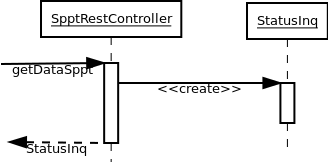
\includegraphics[width=0.8\textwidth]{./resources/uml/uml-seq-inq-thn-not-valid}
  \caption{Diagram \textit{Sequence} Kegagalan \textit{Inquiry} Karena Tahun Pajak Mengandung Karakter Bukan Angka}
  \label{fig:uml-seq-inq-thn-not-valid}
\end{figure}

Objek yang saling berhubungan memang hanya 2 (dua) saja untuk sekenario ini, karena seleksi terhadap karakter pada parameter tahun pajak diperiksa 

\subsection{Skenario \textit{Inquiry} Gagal Karena Data Tidak Ditemukan}

Pada skenario ini, \textit{client} mengirimkan \textit{request} tetapi ada kesalahan bahwa tahun pajak yang di-\textit{request} oleh \textit{client} mengandung karakter bukan angka. Diagram \textit{sequence} dari skenario ini seperti terlihat pada gambar \ref{fig:uml-seq-inq-not-any} :

\begin{figure}[H] 
  \centering
  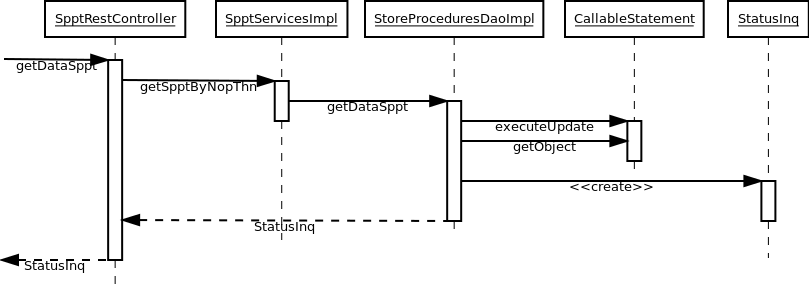
\includegraphics[width=1\textwidth]{./resources/uml/uml-seq-inq-not-any}
  \caption{Diagram \textit{Sequence} Kegagal \textit{Inquiry} Karena Data Tidak Ada Dalam Basis Data}
  \label{fig:uml-seq-inq-not-any}
\end{figure}

Pada diagram \textit{sequence} tersebut, permintaan atau \textit{request} dari \textit{client} akan diterima \textit{server} dan diteruskan oleh \textit{framework} Spring ke \textit{method} getDataSppt milik kelas SpptRestController.

Kemudian \textit{method} getDataSppt akan memanggil \textit{method} getSpptByNopThn milik kelas SpptServicesImpl, yang didalamnya hanya memanggil \textit{method} getDataSppt milik kelas StoreProceduresDaoImpl.

Didalam \textit{method} getDataSppt milik kelas StoreProceduresDaoImpl, terdapat proses koneksi ke basis data melalui kelas CallableStatement, yang pertama melakukan pemanggilan \textit{method} executeUpdate milik untuk mengeksekusi atau memanggil \textit{store procedure} milik basis data, kemudian mengambil nilai balikkannya melalui \textit{method} getObject.

Terakhir adalah melakukan pemeriksaan terhadap nilai balikan dari pembanggil \textit{store procedure} milik basis data, bila nilai kembalian nihil, maka \textit{method} getDataSppt akan membuat instan dari kelas StatusInq, kemudian nilainya dikembalikan ke kelas SpptRestController yang tentu saja dikirimkan hasilnya ke \textit{client}.

\subsection{Skenario \textit{Inquiry} Gagal Karena Kesalahan Server}

Pada skenario ini, \textit{client} melakukan \textit{request inquiry} ke \textit{server}, namun karena beberapa hal, komunikasi antara \textit{server} basis data dan \textit{server} aplikasi mengalami gangguan, sehingga proses \textit{inquiry} gagal dan mengirimkan pesan ke \textit{client} bahwa \textit{request} yang dikirimkan telah gagal diproses. Gambar Diagram \textit{sequence} dari skenario ini dapat dilihat seperti pada gambar \ref{fig:uml-seq-inq-db-error} :

\begin{figure}[H]
  \centering
  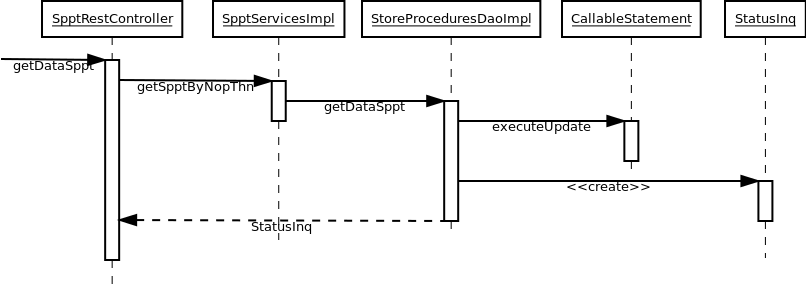
\includegraphics[width=1\textwidth]{./resources/uml/uml-seq-inq-db-error}
  \caption{Diagram \textit{Sequence} Untuk Proses \textit{Inquiry} Yang Gagal Karena Kesalahan Server}
  \label{fig:uml-seq-inq-db-error}
\end{figure}

Diagramnya terlihat sama dengan skenario sebelumnya, yaitu \textit{inquiry} yang gagal karena datanya tidak ada, yang membedakan adalah pada saat \textit{method} getDataSppt milik kelas StoreProceduresDaoImpl melakukan pemanggilan \textit{store procedure} milik basis data melalui \textit{method} executeUpdate pada kelas CallableStatement ada kesalahan, sehingga \textit{method} getDataSppt milik kelas StoreProceduresDaoImpl membuat instan dari kelas StatusInq dan mengembalikannya ke kelas SpptRestController yang kemudian menjadi respon yang dikirim ke \textit{client} sebagai informasi bahwa \textit{request} yang dikirimkan ke \textit{server} gagal diproses.

\subsection{Skenario \textit{Inquiry} Sukses}

Untuk alur proses \textit{inquiry} yang sukses, diagram \textit{sequence}-nya dapat dilihat seperti pada gambar \ref{fig:uml-seq-inq} :
  
  \begin{figure}[H]
    \centering
    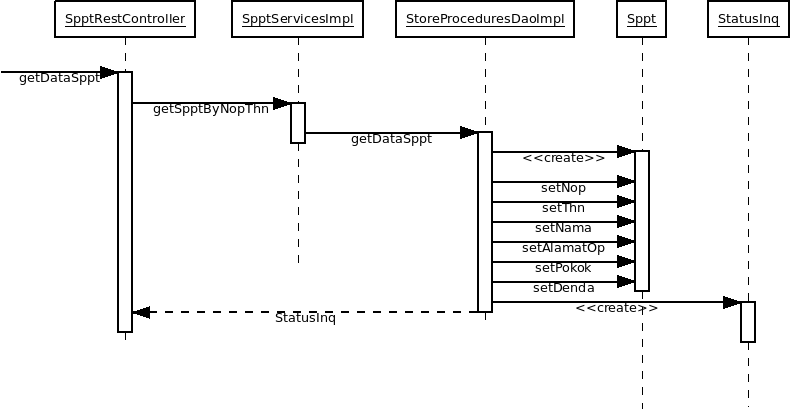
\includegraphics[width=1\textwidth]{./resources/uml/uml-seq-inquiry}
    \caption{Diagram \textit{Sequence} Untuk Menangani \textit{Request Inquiry}}
    \label{fig:uml-seq-inq}
  \end{figure}
  
  Seperti awal dari setiap proses \textit{request} Rest, pada fungsi \textit{inquiry} ini pun berawal dari kelas SpptRestController. Kelas SpptRestController ini kemudian menyalurkannya ke kelas SpptServicesImpl dengan memanggil \textit{method} getSpptByNopThn. Di dalam \textit{method} getSpptByNopThn, kelas SpptServicesImpl memanggil \textit{method} getDataSppt milik kelas StoreProceduresDaoImpl.
  
  Pada kelas StoreProceduresDaoImpl, \textit{method} getDataSppt melakukan koneksi ke basis data dan menampung hasilnya pada kelas Sppt. Hasil-hasil yang diperoleh dari basis data berupa NOP, Tahun Pajak, Nama Wajib Pajak, Alamat Objek Pajak, Besarnya tagihan pokok, dan besarnya Denda Administrasi. Semuanya ditampung yang ditandai dengan pemanggilan \textit{method} setNop, setThn, setNama, setAlamatOp, setPokok, dan setDenda.
  
  Sebelum dikirimkan kembali ke \textit{client}, maka data atau informasi yang ditampung dalam kelas Sppt dipaketkan dengan kelas StatusInq, yang hasilnya dikembalikan ke \textit{client} dalam bentuk kelas StatusInq.

\subsection{Skenario Transaksi Pembayaran Gagal Karena Jam Pembayaran Melebihi Jam Pencatatan}

Pada skenario ini, \textit{request} transaksi yang dikirimkan oleh \textit{client} gagal dilakukan karena waktu pada saat dilakukan pembayaran oleh wajib pajak ke tempat pembayaran, lebih dari waktu dilakukan pencatatan ke basis data. Kondisi ini tidak bisa diterima, karena seharusnya tanggal pencatatan transaksi ke basis data harus lebih terkini dibandingkan kondisi jam bahkan tanggal dilakukan pembayaran oleh wajib pajak.

Diagram \textit{sequence} yang menggambarkan skenario ini seperti terlihat pada gambar \ref{fig:uml-seq-trx-tgl-bayar-error} :

\begin{figure}[H]
  \centering
  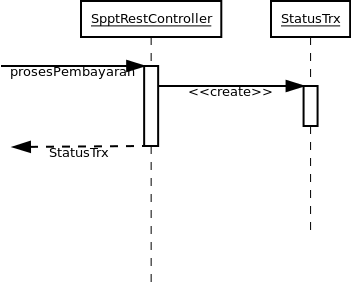
\includegraphics[width=0.75\textwidth]{./resources/uml/uml-seq-trx-tgl-bayar-error}
  \caption{Diagram \textit{Sequence} Transaksi Pembayaran Yang Gagal Karena Jam Pembayaran Melebihi Jam Pencatatan}
  \label{fig:uml-seq-trx-tgl-bayar-error}
\end{figure}

Skenario ini terlihat sederhana karena pemeriksaan tanggal pembayaran dilakukan pada \textit{method} prosesPembayaran milik kelas SpptRestController, \textit{method} inilah yang melakukan tugasnya pada saat ada \textit{request} transaksi pembayaran dari \textit{client}.

Setelah ada kesalahan tanggal pembayaran, \textit{method} ini akan mengirimkan nilai dari kelas StatusTrx sebagai informasi bagi \textit{client} bahwa transaksi yang dikirimkan gagal dilakukan pencatatan pembayaran karena jam dan tanggal pembayaran lebih dari tanggal dan jam sekarang.

\subsection{Skenario Transaksi Pembayaran Gagal Karena Tagihan Telah Terbayar Atau Nihil}

Skenario ini akan menggambarkan pencatatan transaksi pembayaran yang gagal dilakukan karena tagihan telah terbayar atau tagihan nihil. Diagram \textit{sequence} dari skenario ini dapat dilihat pada gambar \ref{fig:uml-seq-trx-nihil} :

\begin{figure}[H]
  \centering
  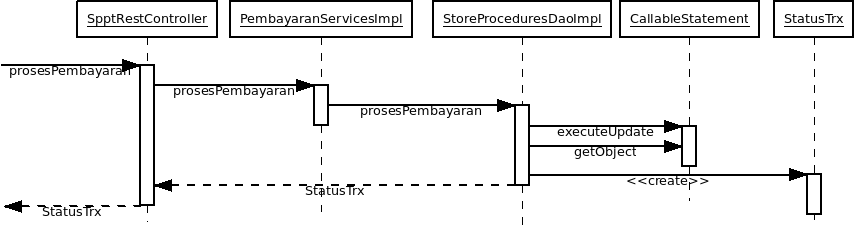
\includegraphics[width=1\textwidth]{./resources/uml/uml-seq-trx-nihil}
  \caption{Diagram \textit{Sequence} Untuk Transaksi Pencatatan Pembayaran Yang Gagal Karena Tagihan Telah Terbayar Atau Nihil}
  \label{fig:uml-seq-trx-nihil}
\end{figure}

Seperti setiap \textit{request} yang diterima dari \textit{client} oleh \textit{server}, bahwa \textit{request} akan diterima oleh kelas SpptRestController, dan untuk \textit{request} transaksi pembayaran akan ditangani oleh \textit{method} prosesPembayaran milik kelas SpptRestController.

Dalam \textit{method} prosesPembayaran pada kelas SpptRestController akan memanggil \textit{method} prosesPembayaran milik PembayaranServicesImpl yang dalam \textit{method} ini pula memanggil \textit{method} dengan nama yang sama, yaitu prosesPembayaran, tetapi milik kelas StoreProceduresDaoImpl.

Kelas StoreProceduresDaoImpl ini akan menghubungkan aplikasi dengan \textit{server} basis data, dengan melakukan pemanggilan pada \textit{method} executeUpdate milik kelas \textit{CallableStatement}, yang hasilnya dapat diambil dengan \textit{method} getObject.

Bila hasil respon dari \textit{server} basis data berupa kode 01, maka artinya, data tersebut telah terbayar, atau status tagihan untuk nomor objek yang diminta nihil, sehingga dalam \textit{method} prosesPembayaran milik kelas storeProceduresDaoImpl ini akan membuat instan dari kelas StatusTrx dan mengirimkannya kembali ke kelas SpptRestController sehingga kelas SpptRestController akan memberikan respon berupa kelas StatusTrx ke \textit{client} sebagai informasi bahwa \textit{request} pencatatan pembayaran telah gagal karena objek pajak yang diminta telah terbayar, atau tidak ada tagihan sama sekali.

\subsection{Skenario Transaksi Pembayaran Gagal Karena Telah Dibatalkan}

Skenario ini akan menggambarkan sebuah \textit{request} pencatatan transaksi pembayaran dari \textit{client} gagal karena objek pajak yang diminta status penagihannya telah dibatalkan. Diagram \textit{sequence} untuk skenario ini dapat dilihat pada gambar \ref{fig:uml-seq-trx-batal} :

\begin{figure}[H]
  \centering
  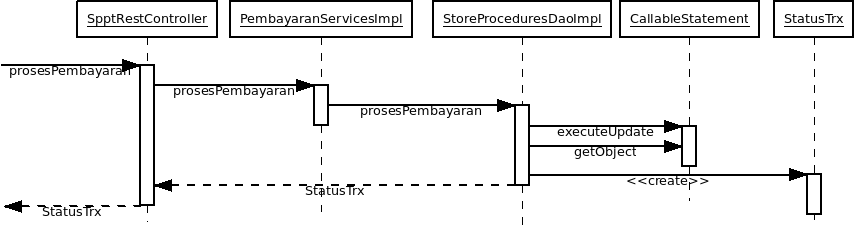
\includegraphics[width=1\textwidth]{./resources/uml/uml-seq-trx-batal}
  \caption{Diagram \textit{Sequence} Untuk Transaksi Pembayaran Yang Gagal Karena Penagihan Atas Objek Pajak Telah Dibatalkan}
  \label{fig:uml-seq-trx-batal}
\end{figure}

Terlihat mirip dengan skenario sebelumnya, dan memang \textit{sequence} menggambarkan kondisi yang sama, yang membedakan adalah pada saat pemanggilan \textit{method} getObject dari kelas CallableStatement, \textit{server} basis data akan memberikan kode '04' yang artinya data penagihan untuk objek pajak yang diminta telah dibatalkan.

Tentunya \textit{client} mengetahui hal tersebut, karena \textit{server} akan mengirimkan kelas StatusTrx yang berisi informasi kegagalan melalui kelas SpptRestController.

\subsection{Skenario Transaksi Pembayaran Gagal Karena Kesalahan Server}

Pada skenario ini, pesan transaksi yang diminta oleh \textit{client} sampai ke \textit{server}, namun pada saat \textit{server} akan melakukan komunikasi dengan basis data terjadi kegagalan. Skenario kegagalan ini dapat dilihat pada gambar \ref{fig:uml-seq-trx-db-error} :

\begin{figure}[H]
  \centering
  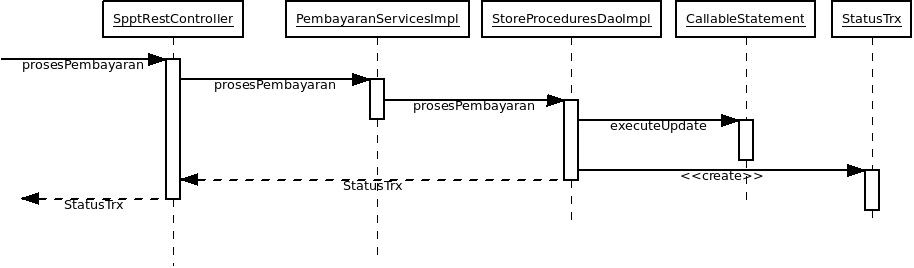
\includegraphics[width=1\textwidth]{./resources/uml/uml-seq-trx-db-error}
  \caption{Diagram \textit{Sequence} Untuk Pencatatan Transaksi Pembayaran Yang Gagal Karena Kesalahan \textit{Server}}
  \label{fig:uml-seq-trx-db-error}
\end{figure}

Transaksi ini diawal dari \textit{request client} yang masuk ke \textit{method} prosesPembayaran milik kelas SpptRestController. Kemudian secara berurutan memanggil \textit{method} prosesPembayaran milik kelas PembayaranServicesImpl dan \textit{method} prosesPembayaran milik kelas StoreProceduresDaoImpl.

Pada \textit{method} prosesPembayaran milik kelas StoreProceduresDaoImpl, saat melakukan pemanggilan \textit{store procedures} dengan \textit{method} executeUpdate milik kelas CallableStatement, terjadi kesalahan komunikasi antara \textit{server} aplikasi dengan \textit{server} basis data, sehingga proses terlempar ke \textit{exception} dan dilakukan pembuatan instan kelas StatusTrx oleh kelas StoreProceduresDaoImpl, dan dikembalikan ke kelas SpptRestController dalam bentuk kelas StatusTrx dan disampaikan ke \textit{client}.

\subsection{Skenario Transaksi Pembayaran Sukses}

Skenario ini menggambarkan alur transaksi pencatatan pembayaran yang sukses dilakukan dan informasinya disampaikan ke \textit{client}. Diagram \textit{sequence} untuk menggambarkan skenario ini seperti terlihat pada gambar \ref{fig:uml-seq-trx} :

\begin{figure}[H]
  \centering
  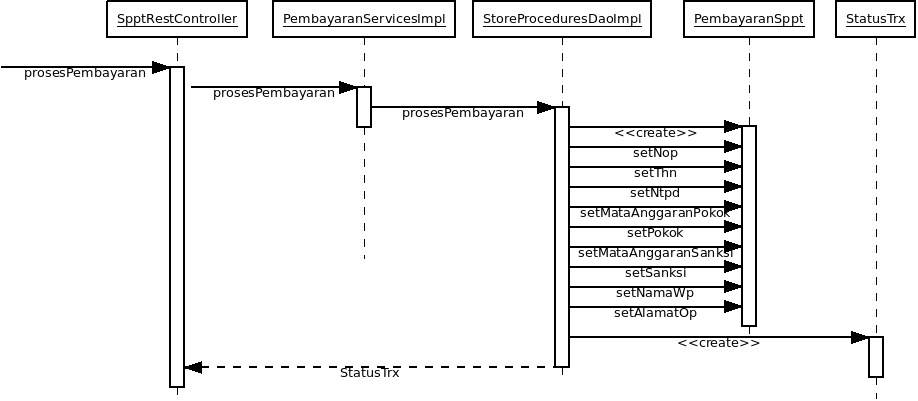
\includegraphics[width=1\textwidth]{./resources/uml/uml-seq-trx}
  \caption{Diagram \textit{Sequence} Pencatatan Transaksi Pembayaran Yang Sukses}
  \label{fig:uml-seq-trx}
\end{figure}

Skenario ini diawali dari pemanggilan \textit{method} prosesPembayaran milik kelas SpptRestController, karena \textit{method} ini lah yang menjadi tempat masuk seluruh proses dari fitur yang ditawarkan oleh \textit{server web services} ini.

Secara berurut, \textit{method} prosesPembayaran milik kelas SpptRestController, akan memanggil \textit{method} prosesPembayaran milik kelas PembayaranServicesImpl, yang didalam \textit{method} ini akan memanggil \textit{method} prosesPembayaran milik kelas StoreProceduresDaoImpl.

Di dalam \textit{method} prosesPembayaran milik kelas StoreProceduresDaoImpl, proses pemanggilan \textit{method} executeUpdate milik kelas CallableStatement dilakukan untuk mengeksekusi \textit{store procedures} pada basis data, kemudian mengambil hasil nilainya dengan memanggil \textit{method} getObject.

Selanjutnya, dari nilai-nilai yang dikembalikan oleh \textit{store procedures} basis data, nilai-nilai tersebut ditampung pada kelas PembayaranSppt, yang kemudian dimasukkan ke dalam kelas StatusTrx untuk dikembalikan ke kelas SpptRestController. Kemudian kelas SpptRestController mengirimkan kelas StatusTrx sebagai respon dari \textit{request} yang dikirimkan oleh \textit{client}.

\subsection{Skenario \textit{Reversal} Gagal Karena Data Yang Diminta Tidak Ada}

Skenario ini menggambarkan proses permintaan \textit{reversal} yang gagal karena data yang diminta untuk dilakukan proses \textit{reversal} tidak ada dalam basis data.

Diagram \textit{sequence} dari skenario ini seperti terlihat pada gambar \ref{fig:uml-seq-rev-null} :

\begin{figure}[H]
  \centering
  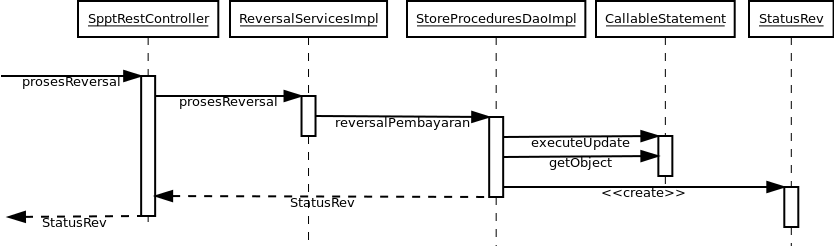
\includegraphics[width=1\textwidth]{./resources/uml/uml-seq-rev-null}
  \caption{Diagram \textit{Sequence Reversal} Yang Gagal Karena Data Tidak Ada Dalam Basis Data}
  \label{fig:uml-seq-rev-null}
\end{figure}

Proses ini berawal dari \textit{request} yang disampaikan oleh \textit{client} yang kemudian diterima oleh \textit{method} prosesReversal milik kelas SpptRestController.

Di dalam \textit{method} prosesReversal milik kelas SpptRestController akan memanggil \textit{method} prosesReversal milik kelas ReversalServicesImpl, yang di dalam \textit{method} ini memanggil \textit{method} reversalPembayaran milik kelas StoreProceduresDaoImpl.

Pada \textit{method} reversalPembayaran milik kelas StoreProceduresDaoImpl ini, akan mengeksekusi \textit{store procedure} milik basis data dengan memanggil \textit{method} executeUpdate milik kelas CallableStatement, dan mengambil nilai hasil eksekusinya melalui \textit{method} getObject.

Hasil dari basis data yang kosong inilah menjadi dasar respon bahwa data yang diminta untuk dilakukan proses \textit{reversal} tidak ada dalam basis data, kemudian \textit{method} reversalPembayaran akan membuat instan dari kelas StatusRev dan mengembalikannya ke kelas SpptRestController, sehingga \textit{server} akan memberikan respon ke \textit{client} berupa kelas StatusRev ini.

\subsection{Skenario \textit{Reversal} Gagal Karena Ada Data Pembayaran Yang Tercatat Ganda}

Skenario ini akan menjelaskan bagaimana proses \textit{request reversal} yang gagal karena adanya pembayaran ganda yang tercatat dalam basis data. Diagram \textit{sequence} untuk skenario ini sama persis dengan kondisi skenario proses \textit{reversal} yang gagal karena data yang diminta tidak ada. Ini karena baik respon terhadap pencatatan pembayaran ganda dan tidak ada data berasal dari \textit{store procedure} milik basis data, sehingga diagram \textit{sequence} akan nampak sama, tetapi respon datanya berbeda.

Diagram \textit{sequence} untuk skenario ini seperti pada gambar \ref{fig:uml-seq-rev-double} :

\begin{figure}[H]
  \centering
  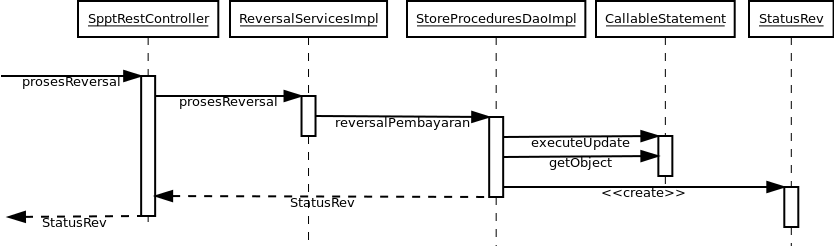
\includegraphics[width=1\textwidth]{./resources/uml/uml-seq-rev-null}
  \caption{Diagram \textit{Sequence} Untuk Proses \textit{Reversal} Yang Gagal Karena Data Pembayaran Tercatat Ganda}
  \label{fig:uml-seq-rev-double}
\end{figure}

Proses ini berawal dari pemanggilan \textit{method} prosesReversal milik kelas SpptRestController, dan alur yang sama seperti skenario proses \textit{reversal} yang gagal karena data yang diminta tidak ada, yang membedakan adalah pada saat pemanggilan \textit{method} getObject milik kelas CallableStatement, respon yang diberikan oleh \textit{store procedure} berbeda dari skenario sebelumnya.

Sebagai respon dari \textit{server} untuk \textit{client}, maka dibentuklah instan dari kelas StatusRev untuk membungkus informasi status proses \textit{reversal} yang terjadi.

\subsection{Skenario \textit{Reversal} Gagal Karena Kesalahan Server}

Skenario ini menjelaskan alur proses \textit{reversal} yang gagal karena ada kesalahan komunikasi antara \textit{server} Rest dengan \textit{server} basis data. Diagram \textit{sequence} dari skenario ini seperti terlihat pada gambar \ref{fig:uml-seq-rev-db-error} :

\begin{figure}[H]
  \centering
  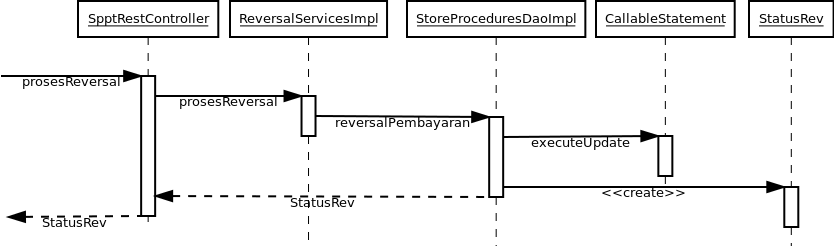
\includegraphics[width=1\textwidth]{./resources/uml/uml-seq-rev-db-error}
  \caption{Diagram \textit{Sequence} Dari Proses \textit{Reversal} Yang Gagal Karena Kesalahan Komunikasi Dengan Basis Data}
  \label{fig:uml-seq-rev-db-error}
\end{figure}

Diagram ini pun terlihat mirip dengan skenario-skenario \textit{reversal} yang gagal sebelumnya, hanya perbedaannya pada saat \textit{method} reversalPembayaran milik kelas StoreProceduresDaoImpl memanggil \textit{method} executeUpdate milik kelas \textit{CallableStatement} ada kesalahan yang tidak diharapkan, sehingga proses keluar melalui \textit{exception}, yang akhirnya \textit{method} reversalPembayaran milik kelas StoreProceduresDaoImpl membuat instan kelas StatusRev, dan menjadi nilai kembalian untuk kelas SpptRestController yang selanjutnya menjadi respon \textit{server} terhadap \textit{request} dari \textit{client}.

\subsection{Skenario \textit{Reversal} Sukses}

Skenario ini akan menjelaskan proses \textit{reversal} yang berhasil. Diagram \textit{sequence} untuk menggambarkan skenario ini adalah seperti pada gambar \ref{fig:uml-seq-rev} :
  
  \begin{figure}[H]
    \centering
    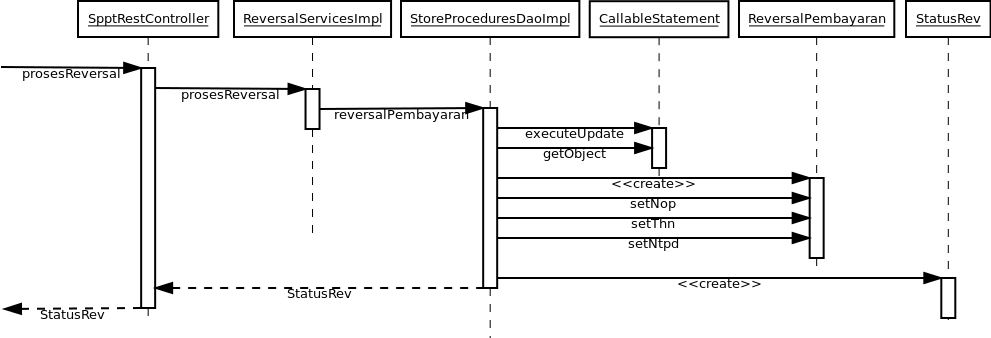
\includegraphics[width=1\textwidth]{./resources/uml/uml-seq-rev}
    \caption{Diagram \textit{Sequence} Untuk Fungsi \textit{Reversal}}
    \label{fig:uml-seq-rev}
  \end{figure}
  
Seperti beberapa \textit{request} sebelumnya, \textit{request reversal} yang sukses ini pun akan dimulai dari kelas SpptRestController pada \textit{method} prosesReversal.
  
Pada \textit{method} prosesReversal kelas SpptRestController akan memanggil \textit{method} yang sama namanya, yaitu \textit{method} prosesReversal tetapi milik kelas ReversalServicesImpl.
  
 Dari \textit{method} prosesReversal milik kelas ReversalServicesImpl ini, kemudian akan memanggil \textit{method} reversalPembayaran pada kelas StoreProceduresDaoImpl yang didalamnya memuat koneksi ke basis data kemudian memanggil \textit{store procedure} dengan menggunakan \textit{method} executeUpdate milik kelas CallableStatement, dan mengambil nilai balikkan dari basis data dengan \textit{method} getObject milik kelas CallableStatement juga yang hasilnya ditampung pada kelas ReversalPembayaran.
  
Pada langkah terakhir, \textit{method} reversalPembayaran kelas StoreProceduresImpl ini akan membungkus kelas ReversalPembayaran di dalam kelas StatusRev yang dikembalikan ke kelas SpptRestController agar dijadikan bahan respon terhadap \textit{request} yang dilakukan oleh \textit{client}.

